\section{Background}

The solution of Lengyel \textit{et al.} \cite{lengyel2010voxel} is
based on extracting an adaptive triangulated surface by applying MC on
an octree.  However, due to its recursive nature, the octree is not
suited for the GPU pipeline.  Hence, to take full advantage ofthe GPU,
we must convert this tree to a non recursive structure.  Such
representations were first introduced by Gargantini
\cite{gargantini1982effective} and are known as linear quadtrees.
They have been implemented on the GPU by Dupuy \textit{et al.}
\cite{dupuy2014quadtrees}.  Along with this implementation, they
presented a LoD criterion that bounds the projected size of the tree
cells.

\subsection{Adaptive surface extraction}

\begin{figure}
\centering
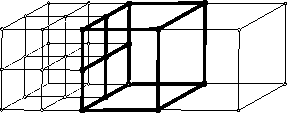
\includegraphics[width=0.8\linewidth]{transition_cell}
\caption{ Triangulating a hierarchical grid with MC creates cracks at level changes.
To fix those, Lengyel \textit{et al}. inserts transition cells (bold).
Those cells are more subdivided on one side to patch the change of resolution.}
\label{transition_cell}
\end{figure}


\paragraph{}
Lengyel \textit{et al}. \cite{lengyel2010voxel} developed a solution to visualise volumetric data in real-time.
They start by subdividing the space with an octree.
At each frame, they select a set of cells within this tree, called the active front, that partitions the space.
The resolution of the partition varies along the space, depending on the chosen cells.
This idea is illustrated for quadtrees in the Figure \ref{fig_quadtree_partitionning}.
Whether a cell is part of this active front is determined by evaluating a LoD criterion.
The selected cells can finally be triangulated using a method similar to MC.

\paragraph{}
When two cells of different resolution meet, T-Junctions appear.
They are due to some vertices in the high resolution cells that have no match in the low resolution cell.
The problem is that when using a MC algorithm, those inconsistencies create cracks in the final triangulation.
To fix this, Lengyel \textit{et al.} inserts transition cells (Figure \ref{transition_cell}) where two cells of different level meet.
Those cells are more subdivided one on side than on the other to patch the difference of resolution.
They are then triangulated with a modified MC, producing a crack-free surface for visualisation.
However, it requires having triangulation tables adapted to the unusual structure of the transitions.
It also demands the use of a restricted octree, since the transitions only allow a single level of difference between neighbouring cells.
As the triangulation is based on modified MC, it is data parallel.

\paragraph{}
The adaptivity of the final triangulation is controlled by a LoD criterion.
Lengyel \textit{et al}. use a measure based on the distance between the cell and the camera, which must therefore be re-evaluated every time the camera moves.

\paragraph{}
On the GPU, recomputing the whole active front from the root node would be too expensive.
Instead, we update the tree by merging or splitting the cells.
If this operation could be done on the GPU, it would be possible to extract equ adaptive triangulation entirely on the GPU.
This requires a non recursive representation for the tree, as well as data parallel update operations.
The LoD must also be evaluable during a data parallel process as it controls the partition.
Those properties can be found using linear trees \cite{dupuy2014quadtrees}.


\subsection{Linear Quadtrees}

\begin{figure}
\centering
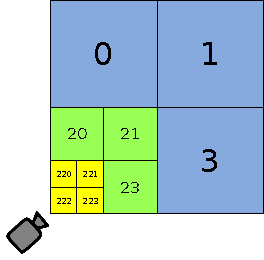
\includegraphics[height=0.17\textheight]{partitioning.pdf}
\hfill
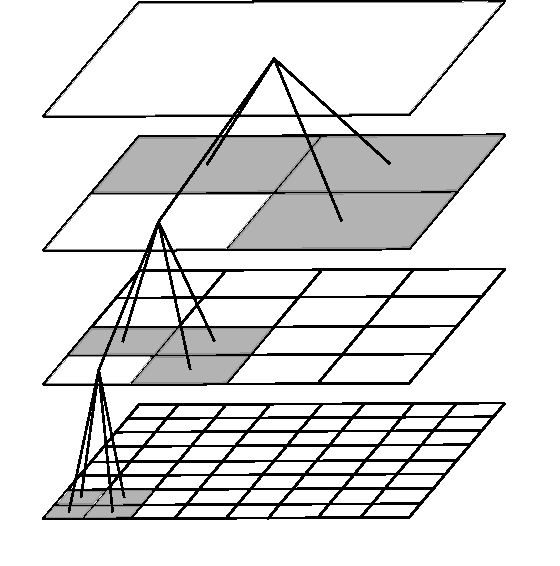
\includegraphics[height=0.17\textheight]{quadtree_activefront}
\caption{In \cite{dupuy2014quadtrees}, a linear quadtree is used to maintain a 2D hierarchical partitioning of space.
(Left) presents such a partitioning.
A cell is more or less subdivided depending on its distance to the camera.
They are also encoded with morton code, that identifies each cell with its position relatively to its parent.
(Right) shows the corresponding active front in the full tree.
This partition is entirely represented by storing the list of codes of the gray cells. }
\label{fig_quadtree_partitionning}
\end{figure}


\paragraph{}
Linear quadtrees were presented by Gargantini \cite{gargantini1982effective} as a non recursive representation for quadtrees.
Such structures were reused by Dupuy \textit{et al.} \cite{dupuy2014quadtrees} who presented a solution to handle them efficiently on the GPU.

\paragraph{}
Linear quadtrees associate a code to each cell, identifying it by its path to the root node.
The full tree is thus entirely represented by the list of its leaves' codes, which removes the recursivity.
In their implementation, Dupuy \textit{et al.} used Morton codes (Figure \ref{fig_quadtree_partitionning}).
Those codes store a spatial position, encoding the location of the cell relatively to its parent.
The final code of a cell is thus the succession of locations between the cell and the root node.
Therefore, the maximal depth of the tree depends on the number of quadrants that can be encoded.
In a quadtree, a cell is divided into $2^2$ quadrants, so encoding one subdivision requires two bits.
Dupuy \textit{et al.} store for each cell its Morton code and its depth within the tree.
Therefore, with a code stored on 32 bits, using 28 bits for the locations and 4 bits for the depth, the tree is limited to 14 levels.

\paragraph{}
Dupuy \textit{et al}. used those quadtrees to maintain a 2D hierarchical space partition.
They thus encode a front of cells within this tree (Figure \ref{fig_quadtree_partitionning}).
To determine if a cell is part of the front, they evaluate on each of them a LoD criterion.
The criterion they chose is view dependent and thus must be evaluated quickly on the GPU.

\paragraph{}
During an update, there a three possible operations on a cell: it can be kept, merged or split.
A merge operation removes the codes of the children's cells from the list and replaces them with the code of the parent cell.
A split operation removes the code of a cell replacing it by the codes of its children.
Therefore, an efficient GPU implementation relies on the fact that those operations can be done independently on each cell.
This is true as long as the LoD criterion is also evaluable independently on each cell.

\paragraph{}
With this implementation of linear tree, it is possible to maintain a quadtree on the GPU.
By generalizing this to the octree, it could be used with the triangulation presented by Lengyel \textit{et al.} to develop a fully data parallel pipeline.
There is however three conditions on the LoD criterion.
It must ensure that the extracted triangles will project onto more than one pixel, to ensure a good rasterization sampling.
The tree must also stay restricted at all times as the transition cells of Lengyel \textit{et al.} only patch cells with a single change in resolution.
Finally, this criterion must allow to detect if the neighbour of a cell is more subdivided than the cell itself in a data parallel manner.
This is mandatory to determine where the transition cells should be inserted.


\subsection{LoD on projected size}

\paragraph{}
When rasterizing a triangulated surface, to ensure a good sampling, all triangles must project onto more than one pixel.
When using a MC algorithm, the size of the generated triangles is bounded by the size of the cell.
Therefore, the cells must all project onto more than one pixel.

\paragraph{}
Dupuy \textit{et al.} \cite{dupuy2014quadtrees} addressed this issue.
They use linear quadtrees to achieve adaptive tessellation.
The subdivision of their quadtree's cells is controlled by a LoD criterion that is evaluable on the GPU and that is based on the cells projected size.
This ensures that all cells project onto more than a pixel.
This criterion is given in equation (\ref{lod_criterion}).
\\
\begin{equation}
s(z) = z \cdot \tan(\alpha)
\label{lod_criterion}
\end{equation}

\paragraph{}
Here, $2 \cdot s(z)$ is the projected screen size at a distance $z$ from the camera, and $2\cdot\alpha$ is the horizontal viewing angle (the fovy). 
To determine if a cell should be merged/split, the ratio $$\frac{\mathrm{cell\_size}}{2 \cdot s(z)}$$ is evaluated.
This ratio is compared to a factor $k$ that controls the density of the triangulation.\\
\begin{equation}
\mathrm{If} \hspace{15pt} \frac{\mathrm{cell\_size}}{2 \cdot s(z)} \geq k \hspace{15pt} \mathrm{then} \hspace{3pt} \mathrm{split}
\label{split_test}
\end{equation}
\begin{equation}
\mathrm{Else} \hspace{3pt} \mathrm{if} \hspace{15pt} \frac{\mathrm{parent\_cell\_size}}{2 \cdot s(z_{\mathrm{parent}})} \leq k \hspace{15pt} \mathrm{then} \hspace{3pt} \mathrm{merge}
\label{merge_test}
\end{equation}
\begin{equation*}
\mathrm{Else} \hspace{3pt} \mathrm{keep}
\end{equation*}
\paragraph{}
Evaluating (\ref{split_test}) splits a cell if its project size exceeds a certain amount.
Equation \ref{merge_test} determines if a cell should merge by testing if the parent of this cell should be split.
This guarantees that all the children of a cell will merge at the same time, since they will all evaluate the criterion on the same parent.
This criterion also maintains a restricted quadtree while the condition $$\frac{\mathrm{cell\_size}}{2 \cdot s(z)} < 2 \cdot k $$ is always verified.
For $k = 2$ , this is ensured as long as the horizontal viewing angle doesn't exceed $142^o$.
We prove this in Appendix 1.

\paragraph{}
This LoD criterion has the four characteristics that we need:
\begin{itemize}
	\item It is data parallel.
	\item It can ensure that the cells project onto more than one pixel.
	\item It maintains a restricted tree.
	\item Its evaluation returns if a cell should split or merge.
\end{itemize}
Therefore, by generalizing it to the octree, we could use it with Lengyel \textit{et al.} triangulation method to implement an adaptive visualisation pipeline on the GPU.
